\chapter{Facility design}
    \section{Version 1} \label{sec:design_v1}

    \section{Version 2} \label{sec:design_v2}

        \subsection{Sizing the double choked LTP thruster}
            \begin{figure}[h]
            \centering
            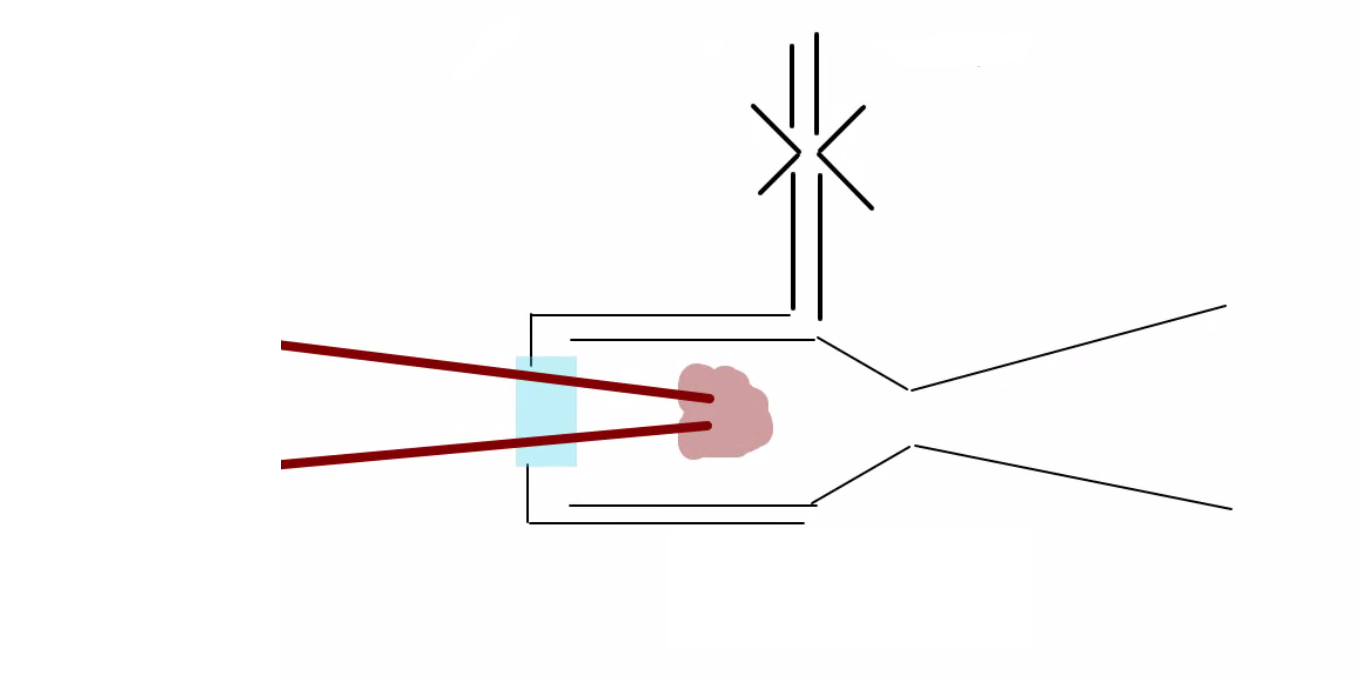
\includegraphics[width=0.8\linewidth]{assets/3 design/double choked sizing.png}
            \caption{\label{fig:frog}Schematic of an LTP thruster.}
            \end{figure}
            
            Let's pose that we have a 300 W power input (laser) and want to run the LTP experiment at 25 bar, with a 50 bar feed pressure. We want the hot gas operation (laser on) to increase the gas' exit velocity to twice that of the cold gas operation (laser off). We will determine together the gas mass flow rate and the diameter of the two orifices needed to choke the flow.
            
            \subsubsection{Cold Ar thuster}
            $C_0$ choked, without nozzle is speed of sound: $323 \:m/s$ This is at ambient temperature (300 K), as we have no laser energy to heat the gas in this case. With a nozzle, we accelerate the gas by $\approx 2$ times. The $v_{exit}$, which is our main performance parameter, is therefore: 
            \[v_{exit} = 646\: m/s\]
            
            \subsubsection{Hot Ar thuster}
            Taking the previous $v_{exit}$ and ionizing the whole flow, we hope that our efficiency is doubled. This gives a $v_{exit}\approx 1300\:m/s$. What nozzle throat size is necessary for this $\dot m$ with $p_{chamber} = 25\: bar$? We know that $MW_{Ar} = 40 \: g/mol$. From Fluids 2, the speed of sound is $c = \sqrt{\gamma R T}$. As we want to double the speed of sound, we are multiplying the temperature by 4! From Thermo 1:
            \[Power = \dot m (h_2-h_1)
            = \dot m C_p (T_2-T_1)\]
            The $C_p$ of argon is $0.520\:kJ/(kg-K)$ Find the $\dot m$ that we can expect in g/s.\vspace{60mm}
            
            Again from Fluids 2, we have the mass flow rate (of an isentropic flow) described by Fliegner's formula:
            \[\frac{\dot m}{A} = p_0\sqrt{\frac{\gamma}{T_0 R}}\frac{M}{(1+\frac{\gamma-1}{2}M^2)^{(\frac{\gamma+1}{2(\gamma-1)})}}\]
            We have a $\gamma = \frac{C_p}{C_v} = 1.666$ for Argon and choked flow at the nozzle. Find the area and the diameter of the circular nozzle.\vspace{170 mm}
            
            We can repeat these calculations for the feed orifice, with the same $\dot m$, a pressure of 50 bar and ambient temperature. This gives us an orifice size of about 0.2 mm, or 10 thou in freedom units.

    
    \section{title}
